%*************************************************
\chapter{Redes Neuronales Artificales}\label{ch:NNBasics}
% ************************************************
\section{Introducción}

En el capítulo anterior se abordaron conceptos básicos del aprendizaje automático, así como dos de sus principales enfoques: aprendizaje supervisado y no supervisado. Las Redes Neuronales Artificiales o ANN's por sus siglas en inglés, son comúnmente un método de aprendizaje supervisado\footnote{Las Redes Neuronales Artificales son algoritmos que también se pueden aplicar en métodos de aprendizaje no supervisado.}, que han tenido gran impulso en los últimos años debido al incremento de datos y a su fácil acceso, así como al crecimiento en poder computacional.
\\
\\
Las \textbf{Redes Neuronales Artificiales}  son algoritmos de aprendizaje automático que simulan\footnote{Las Redes Neuronales Artificiales a menudo son consideradas más como una caricatura de las biológicas, pues su complejidad rebasa el entendimiento e interpretación que se le puede dar a través de los modelos de ANN's.} el mecanismo de aprendizaje de los organismos biológicos, en donde las neuronas, es decir, las células del sistema nerviso, se conectan unas con otras mediante las dedntritas y los axones en la región espacial nombrada sinapsis \autoref{fig:biologicalnn}, en donde las conecciones sinápticas a menudo cambian en respuesta a estimulos externos del organismo, proceso que a grandes rasgos es como aprenden los seres vivos. \cite{Gardell:2010}

\begin{figure}[hb]
  \centering
  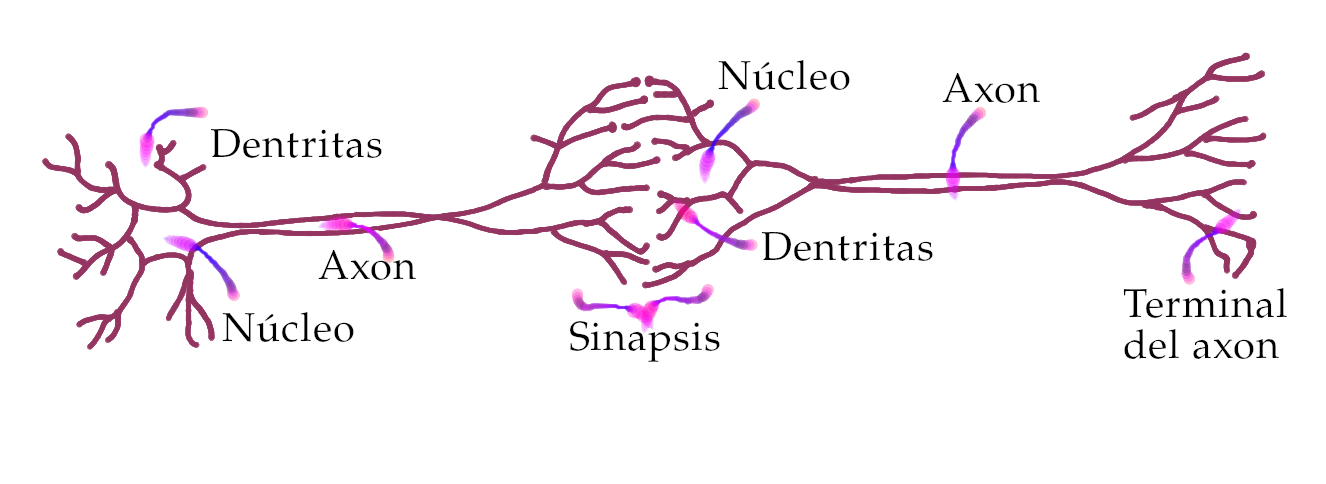
\includegraphics[width=0.75\textwidth]{/home/jessica/Tesis/img/tesis/BioloNN.png}
  \caption{Neuronas biológicas transmitiendo información}
  \label{fig:biologicalnn}
\end{figure}


\section{Arquitectura básica}

\subsection{El Perceptrón}

La \autoref{fig:perceptron} muestra un diagrama de un modelo de Perceptrón, que es el modelo más simple de las ANN's. En este ejemplo la \textbf{capa de entrada} tiene tres componentes:
$$(x_1,x_2,x_3)$$
Es decir, $d=3$ en la \autoref{eq:trainset}. La \textbf{neurona} es la unidad computacional que calcula:

\begin{equation}
  \label{eq:neuronfun}
  f\left( \sum_{i=1}^dw_i\cdot x_i \right)
\end{equation}

donde los $w_i$ son conocidos como los pesos de $x_i$, y $f$ es una función \autoref{sec:FuncAct}.
\begin{figure}[hb]
  \centering
  \begin{tikzpicture}[x=1.5cm, y=1.5cm]
  % Input nodes
  \foreach \i in {1,2,3}
    \node[circle, draw, fill=CTtitle!30] (input\i) at (0,\i) {$x_{\i}$};
  % Summation node
  \node[circle, draw, fill=CTtitle!60, minimum size=1.5cm] (sum) at (2,2) {$\Sigma / f(\Sigma)$};
  % Activation node
  %\node[circle, draw, fill=CTtitle!60, minimum size=1.5cm] (activation) at (4,2) {$f(\Sigma)$};
  % Output node
  \node[circle, draw, fill=CTtitle!30] (output) at (4,2) {$\hat{y}$};
  % Connect the nodes and add weights
  \foreach \i in {1,2,3}
  \draw[->] (input\i) -- node[midway, above] {$w_{\i}$} (sum);
  %\draw[->] (sum) -- (activation);
  \draw[->] (sum) -- (output);

  \node[above, yshift=2.5cm] at (0,2) {Entrada};
  \node[above, yshift=2.5cm] at (2,2) {Neurona};
  \node[above, yshift=2.5cm] at (4,2) {Salida};
  
\end{tikzpicture}

\caption{Diagrama de un modelo simple de Perceptrón}
\label{fig:perceptron}
\end{figure}

El objetivo del algoritmo, es que mediante el entrenamiento de la red \autoref{sec:TrainNN} con un conjunto grande de $M$ datos: $\{\vec{x_j},y_j\}_{j=1}^{M}$ se obtengan los $w_i$ óptimos para que se cumpla:
$$y_l= \hat{y_l} = f\left( \sum_{i=1}^dw_i\cdot x_l \right)$$
con $y_l$ la etiqueta, o valor esperado, correspondiente al vector $\vec{x_l}$, en donde $(\vec{x_l},y_l)$ es un dato que no pertenece al conjunto de entrenamiento que utilizó la red. Esta última propiedad es llamada \textbf{generalización del modelo}.

\subsection{Función de Activación y Función de Pérdida}\label{sec:FuncAct}

\begin{tikzpicture}
  \draw[->] (-2,0) -- (2,0) node[right] {$x$};
  \draw[->] (0,-2) -- (0,2) node[above] {$y$};
  \draw[domain=-1.5:1.5,smooth,variable=\x,CTurl] plot ({\x},{\x});
  %\draw[dashed] (-1.5,-1.5) -- (1.5,1.5);
\end{tikzpicture}


\begin{tikzpicture}
  \draw[->] (-2,0) -- (2,0) node[right] {$x$};
  \draw[->] (0,-2) -- (0,2) node[above] {$y$};
  \draw[CTurl] (-2,0) -- (0,0) node[midway,below right] {$0$} -- (2,2);
\end{tikzpicture}

\begin{tikzpicture}
  \draw[->] (-2,0) -- (2,0) node[right] {$x$};
  \draw[->] (0,-1.5) -- (0,1.5) node[above] {$y$};
  \draw[CTurl] (-2,-1) -- (-0.01,-1) node[left] {-1};
  \draw[CTurl] (0,0) -- (0,1) node[left] {};
  \draw[CTurl] (0,1) -- (2,1) node[right] {1};
\end{tikzpicture}



\subsection{Salida y su Función de Pérdida}

\section{Entrenamiento de una Red Neuronal}\label{sec:TrainNN}
% backpropagation




\subsection{Modelos Multicapa}


\begin{figure}
    \centering
    \begin{tikzpicture}[scale=1.5]
    
    % Input layer
    \foreach \i in {1,...,4}
        \node[circle, draw=black, fill=CTtitle!30] (I-\i) at (0,\i-2) {$x_{\i}$};
    
    % Hidden layer 1
    \foreach \i in {1,...,3}
        \node[circle, draw=black, fill=CTtitle!60] (H1-\i) at (2,\i-1.5) {};
    
    % Hidden layer 2
    \foreach \i in {1,...,3}
        \node[circle, draw=black, fill=CTtitle!60] (H2-\i) at (4,\i-1.5) {};
        
    % Output layer
    \foreach \i in {1,...,2}
        \node[circle, draw=black, fill=CTtitle!90] (O-\i) at (6,\i-1) {$y_{\i}$};
    
    % Connections
    \foreach \i in {1,...,4}
        \foreach \j in {1,...,3}
            \draw[->] (I-\i) -- (H1-\j);
            
    \foreach \i in {1,...,3}
        \foreach \j in {1,...,3}
            \draw[->] (H1-\i) -- (H2-\j);
            
    \foreach \i in {1,...,3}
        \foreach \j in {1,...,2}
            \draw[->] (H2-\i) -- (O-\j);
    
    % Labels
    \node[above, yshift=0.5cm] at (0,2) {Capa de Entrada};
    \node[above, yshift=0.5cm] at (2,2) {Capa oculta 1};
    \node[above, yshift=0.5cm] at (4,2) {Capa oculta 2};
    \node[above, yshift=0.5cm] at (6,2) {Capa de Salida};
    
    \end{tikzpicture}
    \caption{Arquitectura básica de una Red Neuronal Artificial}
    \label{fig:nn}
\end{figure}




\section{Multilayer Perceptron, LSTM ? or other NN maybe}